%LTeX: language=it
\subsection{UC 13 - Modifica evento} \label{sec:UC13}
    \begin{itemize}
        \item \textbf{Attore principale}: MUA;
        \item \textbf{Descrizione}: il MUA deve poter modificare un evento nel sistema;
        \item \textbf{Precondizioni}: l’account che il MUA gestisce è registrato nel sistema, ha un connessione aperta con il sistema ed è autenticato;
        \item \textbf{Postcondizioni}: il MUA modifica l'evento che viene salvato nel sistema;
        \item \textbf{Scenario principale}:
            \begin{enumerate}
                \item il MUA trasmette il nuovo titolo dell'evento (\hyperref[sec:UC13.1]{UC 13.1});
                \item il MUA trasmette la nuova data di inizio dell'evento (\hyperref[sec:UC13.2]{UC 13.2});
                \item il MUA trasmette la nuova data di fine dell'evento (\hyperref[sec:UC13.3]{UC 13.3});
                \item il MUA trasmette la nuova durata dell'evento (\hyperref[sec:UC13.4]{UC 13.4});
                \item il sistema salva l'evento;
            \end{enumerate}
        \item \textbf{Inclusioni}: nessuna;
        \item \textbf{Generalizzazioni}: nessuna;
        \item \textbf{Estensioni}: nessuna.
    \end{itemize}

\begin{figure}[H]
    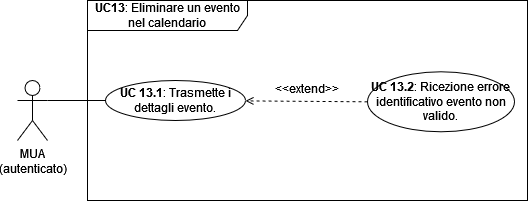
\includegraphics[width=0.813\textwidth]{sections/uc_imgs/UC13.png}
    \centering
    \caption{Diagramma sotto-casi UC 13}
\end{figure}

\subsubsection{UC 13.1 - Trasmette titolo evento} \label{sec:UC13.1}
    \begin{itemize}
        \item \textbf{Attore principale}: MUA;
        \item \textbf{Descrizione}: il MUA trasmette il nuovo titolo per modificare l'evento al sistema;
        \item \textbf{Precondizioni}: il MUA sta usando la funzionalità di modifica di un evento;
        \item \textbf{Postcondizioni}: il sistema conosce il nuovo titolo dell'evento;
        \item \textbf{Scenario principale}:
            \begin{enumerate}
                \item il MUA invia il nuovo titolo per modificare l'evento al sistema;
                \item il sistema controlla che le informazioni ricevute rispettino il seguente requisito minimo:
                    \begin{itemize}
                        \item il titolo dell'evento non è una stringa vuota;
                    \end{itemize}
            \end{enumerate}
        \item \textbf{Inclusioni}: nessuna;
        \item \textbf{Generalizzazioni}: nessuna;
        \item \textbf{Estensioni}:
            \begin{enumerate}[label=\alph*.]
                \item il sistema non riesce a modificare l'evento perché il titolo fornito non è valido:
                \begin{enumerate}[label=\arabic*.]
                    \item il sistema ritorna un errore al MUA di titolo evento non valido (\hyperref[sec:UC13.5]{UC 13.5}).
                \end{enumerate}
            \end{enumerate}
    \end{itemize}



    \subsubsection{UC 13.2 - Trasmette data inizio evento} \label{sec:UC13.2}
    \begin{itemize}
        \item \textbf{Attore principale}: MUA;
        \item \textbf{Descrizione}: il MUA trasmette la nuova data di inizio dell'evento per modificare l'evento al sistema;
        \item \textbf{Precondizioni}: il MUA sta usando la funzionalità di modifica di un evento;
        \item \textbf{Postcondizioni}: il sistema conosce la nuova data di inizio dell'evento;
        \item \textbf{Scenario principale}:
            \begin{enumerate}
                \item il MUA invia la nuova data di inizio dell'evento per modificare l'evento al sistema;
                \item il sistema controlla che le informazioni ricevute rispettino il seguente requisito minimo:
                    \begin{itemize}
                        \item la data di inizio dell'evento è in un formato corretto;
                    \end{itemize}
            \end{enumerate}
        \item \textbf{Inclusioni}: nessuna;
        \item \textbf{Generalizzazioni}: nessuna;
        \item \textbf{Estensioni}:
            \begin{enumerate}[label=\alph*.]
                \item il sistema non riesce a modificare l'evento perché la data di inizio dell'evento fornita non è in un formato corretto:
                \begin{enumerate}[label=\arabic*.]
                    \item il sistema ritorna un errore al MUA di data evento non valida (\hyperref[sec:UC13.6]{UC 13.6}).
                \end{enumerate}
            \end{enumerate}
    \end{itemize}


    \subsubsection{UC 13.3 - Trasmette data fine evento} \label{sec:UC13.3}
    \begin{itemize}
        \item \textbf{Attore principale}: MUA;
        \item \textbf{Descrizione}: il MUA trasmette la nuova data di fine dell'evento per modificare l'evento al sistema;
        \item \textbf{Precondizioni}: il MUA sta usando la funzionalità di modifica di un evento;
        \item \textbf{Postcondizioni}: il sistema conosce la nuova data di fine dell'evento;
        \item \textbf{Scenario principale}:
            \begin{enumerate}
                \item il MUA invia la nuova data di fine dell'evento per modificare l'evento al sistema;
                \item il sistema controlla che le informazioni ricevute rispettino il seguente requisito minimo:
                    \begin{itemize}
                        \item la data di fine dell'evento è in un formato corretto;
                    \end{itemize}
            \end{enumerate}
        \item \textbf{Inclusioni}: nessuna;
        \item \textbf{Generalizzazioni}: nessuna;
        \item \textbf{Estensioni}:
            \begin{enumerate}[label=\alph*.]
                \item il sistema non riesce a modificare l'evento perché la data di fine dell'evento fornita non è in un formato corretto:
                \begin{enumerate}[label=\arabic*.]
                    \item il sistema ritorna un errore al MUA di data evento non valida (\hyperref[sec:UC13.6]{UC 13.6}).
                \end{enumerate}
            \end{enumerate}
    \end{itemize}

    \subsubsection{UC 13.4 - Trasmette durata evento} \label{sec:UC13.4}
    \begin{itemize}
        \item \textbf{Attore principale}: MUA;
        \item \textbf{Descrizione}: il MUA trasmette la nuova durata per modificare l'evento al sistema;
        \item \textbf{Precondizioni}: il MUA sta usando la funzionalità di modifica di un evento;
        \item \textbf{Postcondizioni}: il sistema conosce la nuova durata dell'evento;
        \item \textbf{Scenario principale}:
            \begin{enumerate}
                \item il MUA invia la nuova durata per modificare l'evento al sistema;
                \item il sistema controlla che le informazioni ricevute rispettino il seguente requisito minimo:
                    \begin{itemize}
                        \item la durata dell'evento deve essere consistente con la data di inizio e la data di fine;
                    \end{itemize}
            \end{enumerate}
        \item \textbf{Inclusioni}: nessuna;
        \item \textbf{Generalizzazioni}: nessuna;
        \item \textbf{Estensioni}:
            \begin{enumerate}[label=\alph*.]
                \item il sistema non riesce a modificare l'evento perché la durata fornita non è valido:
                \begin{enumerate}[label=\arabic*.]
                    \item il sistema ritorna un errore al MUA di durata inconsistente (\hyperref[sec:UC13.7]{UC 13.7}).
                \end{enumerate}
            \end{enumerate}
    \end{itemize}


    \subsubsection{UC 13.5 - Ritorna errore titolo evento non valido} \label{sec:UC13.5}
    \begin{itemize}
        \item \textbf{Attore principale}: MUA;
        \item \textbf{Descrizione}: il sistema non riesce a modificare l'evento perché il titolo dell'evento non rispetta i requisiti;
        \item \textbf{Precondizioni}: il MUA ha inviato il titolo dell'evento;
        \item \textbf{Postcondizioni}: il sistema non modifica l'evento, il MUA è stato notificato dell'errore;
        \item \textbf{Scenario principale}:
            \begin{enumerate}
                \item il sistema controlla la sintassi del titolo dell'evento e trova un errore;
                \item il sistema non modifica l'evento e notifica il MUA dell'errore;
            \end{enumerate}
        \item \textbf{Inclusioni}: nessuna;
        \item \textbf{Generalizzazioni}: nessuna;
        \item \textbf{Estensioni}: nessuna.
    \end{itemize}


    \subsubsection{UC 13.6 - Ritorna errore data non valida} \label{sec:UC13.6}
    \begin{itemize}
        \item \textbf{Attore principale}: MUA;
        \item \textbf{Descrizione}: il sistema non riesce a modificare l'evento perché la data non è nel formato corretto;
        \item \textbf{Precondizioni}: il MUA ha inviato il titolo dell'evento;
        \item \textbf{Postcondizioni}: il sistema non modifica l'evento, il MUA è stato notificato dell'errore;
        \item \textbf{Scenario principale}:
            \begin{enumerate}
                \item il sistema controlla il formato della data dell'evento e trova un errore;
                \item il sistema non salva l'evento e notifica il MUA dell'errore;
            \end{enumerate}
        \item \textbf{Inclusioni}: nessuna;
        \item \textbf{Generalizzazioni}: nessuna;
        \item \textbf{Estensioni}: nessuna.
    \end{itemize}

    \subsubsection{UC 13.7 - Ritorna errore durata inconsistente} \label{sec:UC13.7}
    \begin{itemize}
        \item \textbf{Attore principale}: MUA;
        \item \textbf{Descrizione}: il sistema non riesce a modificare l'evento perché la durata non rispetta i requisiti;
        \item \textbf{Precondizioni}: il MUA ha inviato la durata dell'evento;
        \item \textbf{Postcondizioni}: il sistema non modifica l'evento, il MUA è stato notificato dell'errore;
        \item \textbf{Scenario principale}:
            \begin{enumerate}
                \item il sistema controlla la consistenza della durata e trova un errore;
                \item il sistema non modifica l'evento e notifica il MUA dell'errore;
            \end{enumerate}
        \item \textbf{Inclusioni}: nessuna;
        \item \textbf{Generalizzazioni}: nessuna;
        \item \textbf{Estensioni}: nessuna.
    \end{itemize}